\scanpage{15}\mspage{14}
En résumé, en termes de $\unsure{\mathcal{F}|\mathfrak{F}}$, c'est de la donnée de deux \uline{relations} \uline{d'ordre}
\[
% The enclosure reaches the right paper edge without a visible right side.
% Its upper-left corner is open; the lower-left join also has a small gap.
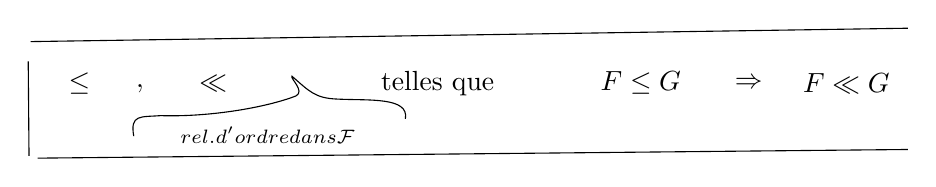
\begin{tikzpicture}[x=1cm,y=1cm,baseline=(ord.base)]
  \draw (0.03,1.48) -- (11.17,1.65);
  \draw (0,1.23) -- (0.01,0.03);
  \draw (0.12,0) -- (11.17,0.11);
  \node (ord) at (0.65,0.95) {$\leq$};
  \node at (1.42,0.88) {$,$};
  \node at (2.35,0.95) {$\ll$};
  \node at (5.20,0.95) {telles que};
  \node at (7.78,0.95) {$F\leq G$};
  \node at (9.15,0.95) {$\Rightarrow$};
  \node at (10.39,0.95) {$F\ll G$};
  \node at (3.04,0.29) {$\scriptstyle\text{rel. d'ordre dans }\mathcal{F}$};
  \draw (1.34,0.28) .. controls (1.29,0.56) and (1.43,0.52) .. (1.68,0.54)
    .. controls (2.33,0.52) and (3.04,0.65) .. (3.40,0.79)
    .. controls (3.52,0.85) and (3.32,1.02) .. (3.35,1.04)
    .. controls (3.57,0.85) and (3.64,0.76) .. (3.93,0.75)
    .. controls (4.32,0.73) and (4.84,0.78) .. (4.79,0.50);
\end{tikzpicture}
\tag*{(1.30)}
\]
que je vais partir.

En termes de celles-ci, on definit \deleted{$\unsure{\mathcal{M}|M}$}
\[
\mathcal{M}\subset\mathcal{F}
\]
par (1.20), avec les relations $\underset{\mathcal{M}}{\leq},\ \underset{\mathcal{M}}{\ll}$ induites par $\underset{\mathcal{F}}{\leq},\ \underset{\unsure{\mathcal{F}|\overline f}}{\ll}$, puis
\[
\mathcal{L}\subset\mathcal{M}
\]
par (1.25). L'application
\[
\mathcal{F}\hookrightarrow\unsure{\mathcal{P}|\mathscr{P}|\mathfrak{P}}(\mathcal{M})\qquad
\mathord{\rlap{$\deleted{X}$}F}\longmapsto\widetilde F=\mathrm{Dep}(F)
\tag*{($*$)}
\]
% The live F is written over the canceled X. The label (*) is retraced.
est \inserted{alors} definie par
\[
\widetilde F=\{X\in\mathcal{M}\mid X\leq F\}
\tag*{(1.31)}
\]
et
\[
\mathcal{F}\hookrightarrow\mathrm{Fig}(\mathcal{M})\qquad
\unsure{\mathord{\rlap{$\deleted{X}$}F}|F}\longmapsto\mathrm{Fig}_{\mathcal{M}}(F)
\tag*{($**$)}
\]
% At this second source token the long rising oblique is clear, but a full
% canceled X cannot be separated from the live F. Both states remain possible.
% No separate predecessor is securely legible beneath the label (**).
par (1.4) :
\[
\mathrm{Fig}_{\mathcal{M}}(F)=\{\widetilde X\mid X\in\widetilde F\}\subset\mathcal{P}(\mathcal{M})
\tag*{\deleted{(1.32)}}
\]
avec
\[
\widetilde X=\{Y\in\mathcal{M}\mid Y\leq X\}\quad.
\]

Ainsi, $\mathcal{F}$ est interprété comme un ens. de parties dans $\mathcal{M}$ via ($*$), et $\leq$ s'interprète simplement par l'inclusion
\[
F\leq G\Longleftrightarrow\widetilde F\subset\widetilde G
\tag*{(1.32)}
\]
